\subsection{Experiment 3}
\label{ssec:exp3}
\addcontentsline{toc}{section}{Experiment 3}

In light of the implementation details provided in section \ref{sec:implem}, this experiment seeks to determine whether there is a linear correlation between the weight of the box and the minimum number of bots required for the task. The settings for this experiment are shown in table \ref{tbl:exp3}.

\begin{table}
 \caption{The variables involved in experiment 3.}
 \begin{center}
  \begin{tabular}{| p{5cm} | c | c |}
   \hline
   \centering \textbf{Variable} & \textbf{Type} & \textbf{Interval} \\ \hline
   gap size & independent & $5$ \\ \hline
   box weight & independent & $[1, 50]$ \\ \hline
   number of bots & independent & $[4, 50]$ with step $5$ \\ \hline
   minimum no. of bots & dependent &  \\ \hline
   runs per parameter set & other & $10$ \\ \hline
  \end{tabular}
 \end{center}
 \label{tbl:exp3}
\end{table}

Fig. \ref{fig:minbots} shows that the number of required bots to move an object of variable weight. Since the gap size is not actually important for this current experiment, it was set to 5 for all the runs concerning it. We can easily see that this minimum number of bots required increased with the weight of the object linearly, independent of the gap size (the averaged results show the same linear dependency, as shown in fig. \ref{fig:minbots}). This is an expected outcome that validates our initial hypothesis since a heavier object would require a higher pushing power that can only be achieved in our model using multiple bots aligned to create the required force. A different approach to the problem would be to modify a bots pushing power, thus leading to a more rapid resolve using less bots. However, we will not consider this possibility during our paper since we have chosen to overlook the physical realism of the individual bots (such is the case in \cite{Yun:2011:OSA:2036628.2036638}).

\restylefloat{minimum_no_bots2}
\begin{figure}[t]
\centerline{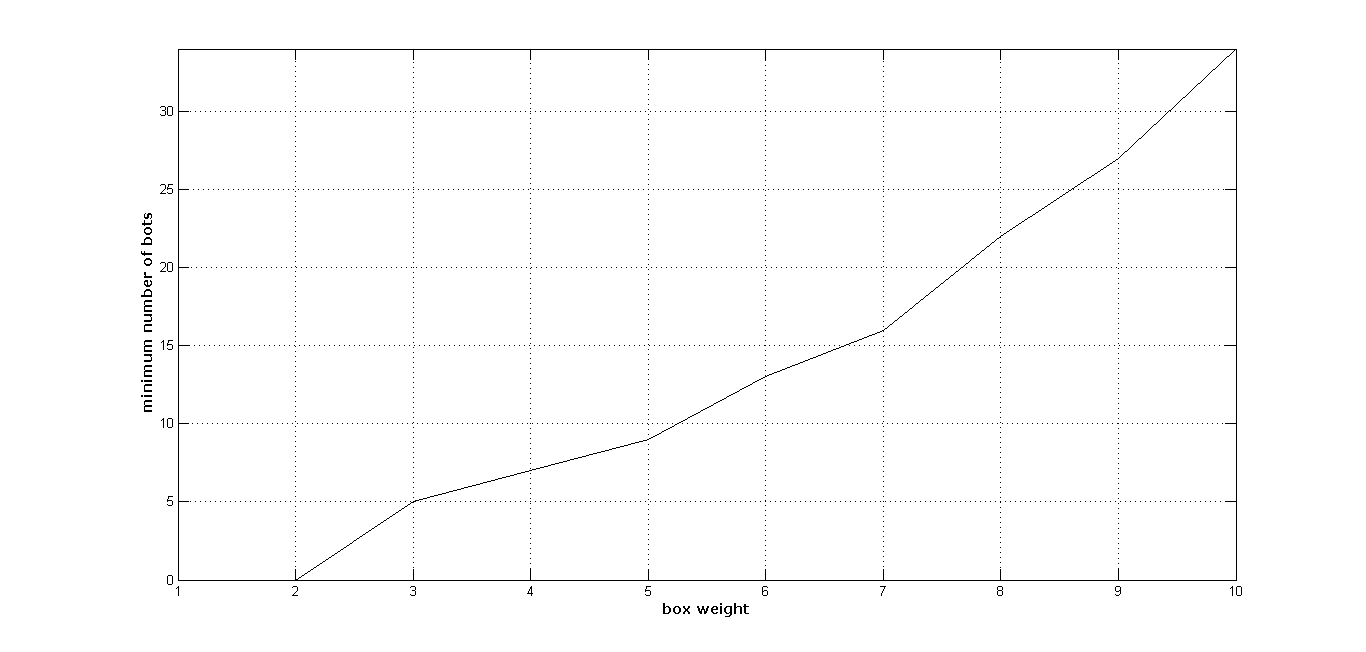
\includegraphics[scale=0.4]{images/minimum_no_bots2}}
\caption{Minimum number of bots required to push a box of a certain weight.}
\label{fig:minbots}
\end{figure}
